% !TeX root = ../../../book.tex
\subsection{好友倾向}\label{sec:section1.4.4}

\subsubsection*{问题描述}

这个问题基于以下一则关于匈牙利社会学家的轶事以及他对儿童朋友圈的观察。

\begin{quote}
    ``20 世纪 50 年代,匈牙利社会学家 S. Szalai 研究了儿童之间的友谊关系。他观察到,在任何大约 $20$ 个孩子的群体中,都能找到四个孩子是共同的朋友,或者四个孩子中没有两个孩子是朋友。在得出社会学结论之前, S. Szalai 咨询了当时三位著名的匈牙利数学家: Erdos, Turan 和 Sos 。简短的讨论后表明,这其实是一种数学现象,而非社会学现象。对于至少 $18$ 个元素上的任意对称关系 $R$,存在 $4$ 个元素的子集 $S$,使得 $R$ 包含 $S$ 中的所有对或不包含其中任何对。这一事实是 1930 年证明的拉姆齐定理(Ramsey's theorem)的一个特例,拉姆齐理论的基础,后来发展成为组合数学的一个丰富领域。 --- (引自麻省理工学院 Jacob Fox 教授的\href{https://www.a.com}{讲义}。)''
\end{quote}

现在我们遵循相同的思路提出类似的问题,但数字较小。具体来说,我们想要找出\emph{满足}其中三人相互都是朋友或敌人的最小群体规模。

\begin{quote}
    假设在一群人中,其中任意两人要么是朋友,要么是敌人,并且这是唯一可能的关系(即没有熟人或亦敌亦友或类似的关系)。以四人为一组,试着为每对指定朋友/敌人关系,使得不会有三人一组都是朋友或敌人。五个人可以实现吗?六个呢?七个?十个?二十个呢?尝试确定最小群体规模,使得你就可以\emph{保证}找到一个由三个人组成的小组,他们要么都是朋友,要么都是敌人。
\end{quote} 

请仔细思考一下,然后再翻页阅读解答。

\clearpage

\subsubsection*{有效地表述问题}

你做出来了吗?这是一个非常棘手的问题,所以如果你没有解出来,请不要感到难过。事实上,我们认为调查这个问题与实际找到答案一样重要,因为有多种方法可以解决这个问题,而且看不同的人如何解释这个问题总是很有趣。

首先,让我们讨论一下如何写下/画出/谈论这种情况。对于该题提出的任何问题,我们都应该考虑一组具有一定规模的人,并思考这群人中任意两人之间的关系。为了解决这个问题,我们需要一种高效且易于解释的方法表示所有这些关系,以便我们可以验证大小为 $3$ 的子群所需的属性。具体来说,我们想要轻松识别是否存在大小为 $3$ 的\emph{同质}子群,即三个人\emph{互为}朋友或\emph{互为}敌人。从现在起,我们将其称为``\textbf{同质性}''。

我们怎么才能做到这一点呢?我们如何才能表示人及其关系呢?我们可以对小组中的人员进行编号,然后写出所有数字对的列表,并用 $F$(朋友)或 $E$(敌人)标记每对数字的关系。让我们尝试为四人小组执行此操作:

\[12F \quad 13E \quad 14F \quad 23F \quad 24E \quad 34F\]

这群朋友/敌人满足同质性吗?验证起来并不那么容易,不是吗?首先,编号使得很难找到大小为 $3$ 的子群,为了验证属性,我们需要检查所有此类子群以确保它们不是 $E E E$ 或 $F F F$。也许在尝试解决问题之前,我们应该找到一种更好的方式来表示信息。对于群体中的所有可能配对,你能想出一种视觉上令人更加愉悦的方式来表示两个人是朋友还是敌人吗?具体来说,我们希望得到一种相对有效的方法来寻找大小为 $3$ 的子群并识别它们是否全是朋友还是全是敌人。

让我们尝试将组中的每个人表示为一个点,并根据这两个人是朋友还是敌人用一种线连接两个人。例如,我们用蓝线表示朋友,用红线表示敌人(记住,任何两个人要么是朋友,要么是敌人,没有别的可能,所以每对点必然有彩色线连接它们)。例如,下图描述了我们在上面分配的关系和符号:

\begin{center}
    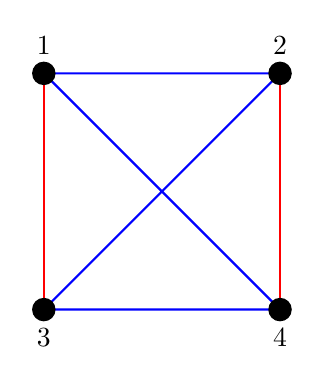
\begin{tikzpicture}[thick,scale=0.5]
        \coordinate (A) at (0,6);
        \coordinate (B) at (6,6);
        \coordinate (C) at (0,0);
        \coordinate (D) at (6,0);
        \draw[blue] (A) node[black, above, yshift=3pt]{$1$}
        -- (B) node[black, above, yshift=3pt]{$2$}
        -- (C) node[black, below, yshift=-3pt]{$3$}
        -- (D) node[black, below, yshift=-3pt]{$4$}
        -- (A);
        \draw[red] (A)--(C);
        \draw[red] (B)--(D);
        \foreach \n in {A,B,C,D}
            \node at (\n)[circle,fill,inner sep=3pt]{};
    \end{tikzpicture}
\end{center}

现在,我们要用什么方法来验证同质性?我们需要三个点(三个人),使得它们之间的所有线都是蓝色(都是朋友)或红色(都是敌人)。没错 --- 我们寻找的正是\textbf{单色三角形}!(注意:我们希望三角形的顶点是我们绘制的原始点;也就是说,我们不希望顶点是两条线的交点。此外,\emph{单色}来自希腊语 \emph{monos} 和 \emph{khroma},分别表示``一个''和``颜色''。)这种表示方式更容易直观地解释,并且可以更快地检验。

根据上图,我们解决了四人组问题:我们找到了朋友和敌人的特定排列,因此不存在全为朋友或全为敌人的三人组。也就是说,不存在具有同质性的大小为 $3$ 的子组。这表明这样的情况可以用四个人来实现,因此我们不能\emph{保证}四个人之间一定存在具有同质性的组。

你还能找到另一个这样的排列吗?你如何确定这与我们已经看到的排列\emph{不同}?有多少种不同的排列满足同质性?现在,尝试绘制一个排列,该排列\emph{一定}具有大小为 $3$ 且具有同质性的子组。那看起来会是什么样?这样的排列有多少种?

\subsubsection*{重述 $n = 5$ 的问题}

让我们继续思考由五个人组成的小组。我们的图需要发生改变,因为我们现在有五个点,这意味着需要绘制更多的线。尽管如此,我们还是会用蓝色或红色线填充所有连接,并确保没有单色三角形。这可能吗?(提示:尝试将点排列成规则的五边形形状,然后填充线。)尝试画几次,看看你的排列是否有效。随机画几条线,然后通过确保添加的新线不会创建单色三角形来指导你的选择,这也可能有帮助。

你做出来了吗?翻页看看我们是如何做的...

\clearpage

\subsubsection*{解答:$n=5$}

这是我们在五个点之间排列的红/蓝线,完全避免了同质性:

\begin{center}
    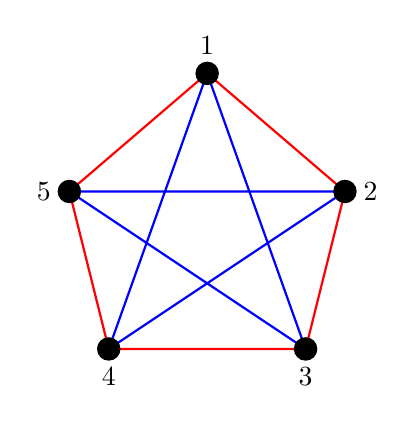
\begin{tikzpicture}[thick,scale=0.5]
        \coordinate (A) at (0,0);
        \coordinate (B) at (5,0);
        \coordinate (C) at (6,4);
        \coordinate (D) at (2.5,7);
        \coordinate (E) at (-1,4);
        \draw[red] (A) node[black, below, yshift=-3pt]{$4$}
        -- (B) node[black, below, yshift=-3pt]{$3$}
        -- (C) node[black, right, xshift=3pt]{$2$}
        -- (D) node[black, above, yshift=3pt]{$1$}
        -- (E) node[black, left, xshift=-3pt]{$5$}
        -- (A);
        \draw[blue] (A)--(D)--(B)--(E)--(C)--(A);
        \foreach \n in {A,B,C,D,E}
            \node at (\n)[circle,fill,inner sep=3pt]{};
    \end{tikzpicture}
\end{center}

请注意该图形优雅的对称性:所有红线均位于五边形的外侧,所有蓝线均位于该形状的内部。这样做的原因是,任意三个相邻点作为顶点的三角形必须使用两条外线和一条内线,任意三个不相邻点作为顶点的三角形必须使用两条内线和一条外线。(想一想:为什么我们不能用三条内线或三条外线来组成一个三角形?)这\emph{保证}了我们绘制的任何三角形都会使用两条不同颜色的线,所以这个图形不具有同质性!当然,我们可以查看图中所有可能的三角形,并确保它们都不使用一种颜色。这样的三角形有多少个?你能多快手工找到所有这些三角形?这样做是否更容易,或者注意我们上面提到的内部/外部属性?

也许你找到的解决方案与我们的图不同。你怎么知道它实际上是否是不同的图形?你的图中有多少条蓝线、多少条红线?我们的图呢?尝试通过移动点来重新绘制图形,但保持点之间的关系(即任意两个点之间绘制的线条的颜色)。你能把你的图形弄得跟我们的一样吗?你认为这对本题解的数量意味着什么?

\subsubsection*{$n=6$ 的情况}

好的,现在我们可以思考六个人的情况了。就点和线而言,我们希望用蓝色或红色线绘制六个点之间所有可能的连接,并确保不存在边都为相同颜色的三角形。在绘制前,请思考四个点和五个点时我们的解决方案。这些解是什么样的?这次我们要画多少线?我们可以试着让这个数字看起来像五个点的解决方案吗?有时,思考当前问题的解决方案与以前工作有何相似之处会大有帮助。现在,尝试画出这个图形,看看会发生什么。

有效吗?为什么无效?你在哪里遇到了麻烦?在不得不绘制单色三角形之前,你可以画多少条线?也就是说,在你绘制下一条线形成单色三角形之前,无论它是蓝色还是红色,你可以向图形中插入多少条线?某种程度上,这些问题对于解决这个特定难题来说是无关紧要的问题,但它们值得思考,因为它们本身很有趣,并且它们可能会引导我们找到这个难题的解决方案或其概括。为了便于说明,这是我们在图形中分配红线和蓝线的一种方案。我们为什么停在这里?还需要添加多少条线?我们能加进去吗?

\begin{center}
    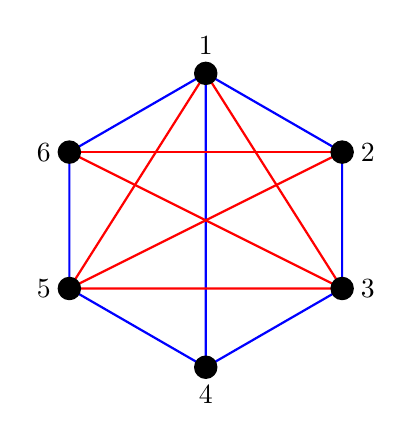
\begin{tikzpicture}[thick,scale=0.5]
        \coordinate (A) at (0,0);
        \coordinate (B) at (-3.4642,2);
        \coordinate (C) at (-3.4642,5.4642);
        \coordinate (D) at (0,7.4642);
        \coordinate (E) at (3.4642,5.4642);
        \coordinate (F) at (3.4642,2);
        \draw[blue] (A) node[black, below, yshift=-3pt]{$4$}
        -- (B) node[black, left, xshift=-3pt]{$5$}
        -- (C) node[black, left, xshift=-3pt]{$6$}
        -- (D) node[black, above, yshift=3pt]{$1$}
        -- (E) node[black, right, xshift=3pt]{$2$}
        -- (F) node[black, right, xshift=3pt]{$3$}
        -- (A)
        -- (D);
        \draw[red] (B)--(E);
        \draw[red] (C)--(F);
        \draw[red] (B)--(D)--(F)--(B);
        \draw[red] (C)--(E);
        \foreach \n in {A,B,C,D,E,F}
            \node at (\n)[circle,fill,inner sep=3pt]{};
    \end{tikzpicture}
\end{center}

我们现在面临的情况很有趣,因为它与我们之前面临的情况性质相反。在四个点和五个点的情况中,我们想表明\emph{可以}通过排列所有线来消除单色三角形。为了证明这一点,只需画出来就好!画出具有所需属性的\emph{特定}图形就足以证明可以实现我们想要的属性。然而,对于六个点,似乎不可能将线条排列得不存在单色三角形。我们怎样才能证明这是事实呢?我们很容易想到,只需考虑线条的所有可能排列,并论证每一中排列中至少有一个单色三角形。这可行吗?线条有多少种排列方式?我们如何在任意给定图形中轻松找到单色三角形?还记得我们对五个点的图形进行此操作吗?我们注意到,任何三角形都必须使用\emph{至少}一条来自外部的线和\emph{至少}一条来自内部的线,这保证了任何三角形都有两种类型的线。我们可以在这里做同样的事情,并明确一些\emph{保证}存在非单色三角形的性质吗?

问题是,图中六点之间线的可能排列方式太多了,我们无法手动完成所有检查!这里有 $15$ 条线需要绘制,每条线都可以是蓝色或红色,因此共有 $2^{15}$ 种可能的排列。这是一个很大的数字!(实际上,排列可能性会稍微少一些,因为其中一些排列在某种意义上是等价的;更专业地说,它们是``\emph{同构的}''。)

\subsubsection*{解答:处理\emph{任意}图形}

我们需要更巧妙地进行论证,这样我们就可以在不绘制特定图形的情况下证明\emph{任意}图形的性质。也就是说,我们需要找到一些事实,一些对所有可能的六点图都成立的性质,但我们仍然能够推断出一定存在三角形。解决这个问题的一种方法是考虑在图形的一小部分中绘制线条。具体来说,让我们取六个点中的任意一个,并考虑从该点引出的五条线。例如,我们可能会得到下面的图形:

\begin{center}
    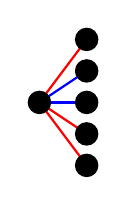
\begin{tikzpicture}[thick,scale=0.2]
        \coordinate (A) at (0,0);
        \coordinate (B) at (3,2);
        \coordinate (C) at (3,0);
        \coordinate (D) at (3,4);
        \coordinate (E) at (3,-2);
        \coordinate (F) at (3,-4);
        \draw[blue] (A)--(C);
        \draw[blue] (A)--(B);
        \draw[red] (A)--(D);
        \draw[red] (A)--(E);
        \draw[red] (A)--(F);
        \foreach \n in {A,B,C,D,E,F}
            \node at (\n)[circle,fill,inner sep=3pt]{};
    \end{tikzpicture}
\end{center}

有多少蓝线,多少红线?这在一定程度上是一个棘手的问题:我们并没有真正考虑任何\emph{特定}图形(如上面的图形),而是试图找到有关所有可能图形的事实。因此,我们不能太具体地回答这个问题。假设我们看到一个\textbf{任意}图形,我们必须提出一个无论该图形是什么都有效的论证。 

我们\emph{可以}这样说:必须至少有三条蓝线或三条红线。你明白为什么这是真的吗?使其不成立的唯一方法是从特定点出发,有两条(或更少)蓝线和两条(或更少)红线,共计四条(或更少)线。不过,我们必须画出所有可能的连接,因此应该有五条!(这个论证是``\emph{抽屉原理}''的一个例子。这个原理说的是,我们无法将两种不同颜色的五个物体放入两个不同盒子中,而不将三个同种颜色的物体放入一个盒子。对这类问题来说,抽屉原理是一个非常有用的策略,我们稍后将在 \ref{sec:section8.6} 节更详细地研究该原理。)

那么我们的立场是什么呢?我们从任意一个六个点、填满线的图形开始,到专注于一个特定的点;从这个点出来,一定有三条蓝线或三条红线。它可以是任意一种颜色,所以我们不能仅仅假设它是红色的并遵循这种假设进行论证;我们可以这样做,但之后必须回到这一点,看看如果这三条线是蓝色的,会发生什么变化。因此,让我们这样处理:让我们检查所有有三条红线从该特定点引出的图形。我们能得到什么?我们还没有对图中的其他线做出任何假设,所以让我们看看它们可能是什么。观察下图,看看到目前为止我们假设存在哪些线条颜色:

\begin{center}
    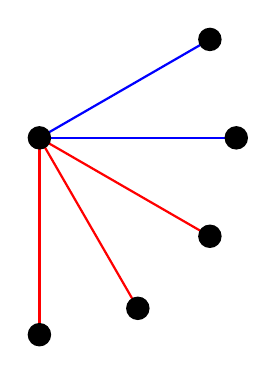
\begin{tikzpicture}[thick,scale=0.5]
        \coordinate (A) at (0,0);
        \coordinate (B) at (4.33,2.5);
        \coordinate (C) at (5,0);
        \coordinate (D) at (4.33,-2.5);
        \coordinate (E) at (2.5,-4.33);
        \coordinate (F) at (0,-5);
        \draw[blue] (A)--(C);
        \draw[blue] (A)--(B);
        \draw[red] (A)--(D);
        \draw[red] (A)--(E);
        \draw[red] (A)--(F);
        \foreach \n in {A,B,C,D,E,F}
            \node at (\n)[circle,fill,inner sep=3pt]{};
    \end{tikzpicture}
\end{center}

现在,可以在该图中添加哪些线而不会在三点之间形成同种颜色的三角形?我们不能对图中两个孤立点之间的线做任何假设,所以让我们关注底部的三个点。其中的线条可能是什么颜色?如果其中任何一条是红色的,那就会在该线的两个端点和我们关注的原始点之间形成一个单色三角形!这是有问题的。

\begin{center}
    \begin{tikzpicture}[thick,scale=0.5]
        \coordinate (A) at (0,0);
        \coordinate (B) at (4.33,2.5);
        \coordinate (C) at (5,0);
        \coordinate (D) at (4.33,-2.5);
        \coordinate (E) at (2.5,-4.33);
        \coordinate (F) at (0,-5);
        \draw[blue] (A)--(C);
        \draw[blue] (A)--(B);
        \draw[red] (A)--(D);
        \draw[red] (A)--(E);
        \draw[red] (A)--(F);
        \draw[red] (E)--(F);
        \draw [red,-stealth,very thick] (-2,-2.4) node[red, above]{$\text{红色三角形}$} -- (1,-3.5);
        \foreach \n in {A,B,C,D,E,F}
            \node at (\n)[circle,fill,inner sep=3pt]{};
    \end{tikzpicture}
\end{center}

避免这种情况的唯一方法是将所有这些线都变成蓝色。但这会在这三个点之间形成一个蓝色三角形!哇,看来无论我们做什么都无法避免生成单色三角形!

\begin{center}
    \begin{tikzpicture}[thick,scale=0.5]
        \coordinate (A) at (0,0);
        \coordinate (B) at (4.33,2.5);
        \coordinate (C) at (5,0);
        \coordinate (D) at (4.33,-2.5);
        \coordinate (E) at (2.5,-4.33);
        \coordinate (F) at (0,-5);
        \draw[blue] (A)--(C);
        \draw[blue] (A)--(B);
        \draw[red] (A)--(D);
        \draw[red] (A)--(E);
        \draw[red] (A)--(F);
        \draw[blue] (F)--(D)--(E)--(F);
        \draw [blue,-stealth,very thick] (5.5,-3.8) node[blue, right]{$\text{蓝色三角形}$} -- (2.5,-3.8);
        \foreach \n in {A,B,C,D,E,F}
            \node at (\n)[circle,fill,inner sep=3pt]{};
    \end{tikzpicture}
\end{center}

让我们回到抽屉原理并重新评估情况。如果原理保证的相同类型的三条线是蓝色而不是红色会怎样?其实,不会有什么改变。向图形底部的三个点之间添加新线,我们仍然会陷入困境:

\begin{center}
    \begin{tikzpicture}[thick,scale=0.5]
        {
            \coordinate (A) at (0,0);
            \coordinate (B) at (4.33,2.5);
            \coordinate (C) at (5,0);
            \coordinate (D) at (4.33,-2.5);
            \coordinate (E) at (2.5,-4.33);
            \coordinate (F) at (0,-5);
            \draw[red] (A)--(C);
            \draw[red] (A)--(B);
            \draw[blue] (A)--(D);
            \draw[blue] (A)--(E);
            \draw[blue] (A)--(F);
            \draw[blue] (E)--(F);
            \draw [blue,-stealth,very thick] (-2,-2.4) node[blue, above]{$\text{蓝色三角形}$} -- (1,-3.5);
            \foreach \n in {A,B,C,D,E,F}
                \node at (\n)[circle,fill,inner sep=3pt]{};
        }
        {
            \coordinate (A1) at (8,0);
            \coordinate (B1) at (12.33,2.5);
            \coordinate (C1) at (13,0);
            \coordinate (D1) at (12.33,-2.5);
            \coordinate (E1) at (10.5,-4.33);
            \coordinate (F1) at (8,-5);
            \draw[red] (A1)--(C1);
            \draw[red] (A1)--(B1);
            \draw[blue] (A1)--(D1);
            \draw[blue] (A1)--(E1);
            \draw[blue] (A1)--(F1);
            \draw[red] (F1)--(D1)--(E1)--(F1);
            \draw [red,-stealth,very thick] (13.5,-3.8) node[red, right]{$\text{红色三角形}$} -- (10.5,-3.8);
            \foreach \n in {A1,B1,C1,D1,E1,F1}
                \node at (\n)[circle,fill,inner sep=3pt]{};
        }
    \end{tikzpicture}
\end{center}

如果我们加入任何蓝色线,它就会与原始点形成一个单色三角形,如果我们将它们全部变成红色,就会在那三个点间形成一个单色三角形!从这个意义上讲,我们在抽屉原理之后遵循的两个论证是\emph{相同的}。如果我们用``红色''替换``蓝色''一词,反之亦然,我们会得到相同的论点。有时,数学家会利用这种情况来简化证明,只说``不失一般性,三条线是红色的''。这通常意味着,如果我们做出其他选择(即,如果线是蓝色的),那么进一步的论证在数学上将具有相同的结构,因此我们可以不重复书写相同的文字来节省时间和空间。事实上,这种情况非常常见,以至于有时你可能会看到``不失一般性''这个短语缩写为 \textbf{WOLOG} 或 \textbf{WLOG}。

\subsubsection*{解答:总结结果}

到目前为止我们取得了什么成果?我们绘制了\emph{特定}的图形,表明我们可以将线条排列在四个和五个点之间,而不出现单色三角形,并且我们认为\emph{任何}由六个点构成的图\emph{一定}具有单色三角形。就题目中朋友/敌人的表述而言,这意味着任何六人组必然存在一个三人组,其中的成员要么都是朋友要么都是敌人。

请注意,把这个问题改写成这个点/线的形式是多么有帮助;它让我们完全忘记了问题的社交背景(某种程度上,这可能会分散注意力),并简化了术语和符号(我们将成对的人标记为``朋友''或``敌人''变为简单地绘制两点之间一条线)。这是一个非常有用的策略:提取谜题的内在结构 --- 底层工作、元素之间的关系、它们如何相互作用等 --- 并根据这些部分重写所有内容。这可以使难题变得更容易理解和解决,并且可以指导我们设计更好的符号。如果我们继续用 $13F, 23E, \dots$ 这种符号来解决这个问题会怎样?也许最终能解决,但会困难得多!

这个题目最初的问题之一是确定一个下界,使得任何更大的人群都必然拥有该子群属性。你认为我们已经做到了吗?我们确定了一个下界了吗?六可能是这个数字吗?为什么是或为什么不是?在任意七人组中,都有一个较小的六人组,而我们上面的工作证明该小组中必然存在三个共同的朋友/敌人!当然,这适用于任何人数超过六人的群体,因此这一定是我们要寻找的精确下界。这与题目原始陈述中提到的结果类似,匈牙利社会学家在规模为四的子群中注意到了这种现象。这个问题解决起来要困难得多,所以我们这里解决了一个更小、更简单的案例。这两个结果都与称为\textbf{拉姆齐理论}的一大类问题有关。组合学和图论的这个分支致力于识别这些``下界'',随着某种结构(如一群人)的规模不断增长,最终会出现一个点,我们可以\emph{保证}找到一个具有某种属性的子群(三个共同的朋友/敌人)。起初被认为是一种社会学现象,后来被证明是严格的数学事实。牛不牛!

\subsubsection*{泛化:留给你的问题}

在继续之前,让我们提出一些有趣且相关的问题。如果我们要寻找不同规模的同质群(例如四个、五个或十二个)该怎么办?当然,总的来说,我们必须有更多的人才能保证找到这样的子群。我们可以一直这样做吗?也就是说,给定任何所需的子群大小,我们可以像上面那样确定一个下界吗?即使没有找到特定的数字,你能想出如何证明这样的下界一定存在吗?此外,如果我们允许第三种可能:朋友、敌人、陌生人,又会怎样呢?我们可以回答关于同质群的类似问题吗?这些都与拉姆齐理论相关,甚至其中一些问题相当难以回答,需要数学家多年努力才能解决。许多此类简单问题仍然是悬而未决的、未解难题!如果你在这些问题上没有任何进展,请不要灰心。我们相信,对这些问题的任何尝试和思考都是有意义且有益的。

\subsubsection*{解题心得}

这个问题带来了几个困难。首先,我们必须找到一种方法来以有意义的方式解释谜题,以便我们可以解决这个问题,这涉及到提出适当的符号来表示题目的元素。这是解决数学问题的重要组成部分,特别是这种不将符号和可视化作为问题陈述一部分的问题。

其次,为了确定 6 是群规模下界,我们必须以某种方式证明某些事情是\emph{不}可能的,但要检验的可能情况数量太大,无法单独检验每种情况。这种情况经常发生,特别是在与计算机科学和算法相关的问题中。为了解决这个问题,我们必须采用一种比大力出奇迹更巧妙的策略,而且并不总是清楚该采取什么策略。在这里,我们先是尝试填入线,就好像它会成功一样,然后意识到我们已经达到了一个无法添加的地步。证明某件事是可能的,相当于只是展示该现象的一个例子(我们对四人和五人组就是这么做的),但证明某件事是\emph{不可能}的可能要棘手得多,并且需要一些依赖上下文的独创性。

最后,我们发现,思考与当前问题密切相关的问题可能会很有趣,这些相关问题往往只需调整原问题的一个或多个条件。如果我们寻找更大的子群怎么办?如果我们允许更多类型的线怎么办?这将如何改变结果?通过改变这些条件来探索问题的边界可以带来新的数学发现和技术,并促使数学家积极探寻新的知识和分享知识的方法。

\clearpage
